%%% Research Diary - Entry
%%% Template by Mikhail Klassen, April 2013

\documentclass[11pt,letterpaper]{article}

\newcommand{\workingDate}{\textsc{2022 $|$ January $|$ 31}}
\newcommand{\userName}{Ganning Xu}
\newcommand{\institution}{Research in \\ Computational Science \\ North Carolina School of Science and Math}
\usepackage{researchdiary_png}
%\usepackage{natbib}
%\bibliographystyle{abbrvnat}
%\setcitestyle{authoryear,open={((},close={))}}
\usepackage{float}
\usepackage{wrapfig}
\usepackage{hyperref}
\usepackage{hyperref}

\begin{comment}
Resources
    Table Generator: https://www.tablesgenerator.com/
    Overleaf Project: https://www.overleaf.com/project/61fc1906472d003c89b4c1f1
    GitHub Project: https://github.com/ganning127/RCompSci_Research_Notebook
\end{comment}

\begin{document}
\univlogo

\section{Week of January 31, 2022}

$\surd$ {\Large \textcolor{red}{RRG Comment:acknowledging notebook establishment } } 

\textbf{Note}: I take a lot of my notes in my \href{https://drive.google.com/drive/folders/17ZhkJZveiDomM2K2MYST_-PhuzrndiVT?usp=sharing}{Google Drive}, so my notebook might not be as detailed.

\subsection{Monday, January 31, 2022}
First day of research in computational science. Went over introductions, course expectations, and how this class would work.

\subsection{Wednesday, February 2, 2022}
Went over how to read request for proposals (RFP) and covered the Research in Computational Science \href{https://drive.google.com/file/d/1cvPQnz40H3bqiEyOdgzRMyYjtK4gxPB5/view?usp=sharing}{RFP}.


We also covered an intro \href{https://drive.google.com/file/d/1hlGEsI95i6WEo5NzAbqjr73ax-MP5L8G/view?usp=sharing}{guide to computational thinking}. Begin by starting with a research question that can be broken down into subproblems. The first subproblem should be "low hanging fruit", while the latter ones should be harder to achieve. Also, it is important to make assumptions when creating the model, as it simplifies it. It's important to be able to distinguish which data is important and which data is not as useful. 

When creating algorithms, you can either use an existing one, modify an existing one, or create your own. Creating your own algorithm is usually difficult. 

\textbf{Important notes}
\begin{itemize}
    \item Letter of intent due on Friday, March 4, 2022 at 5 PM. 
    \item Preliminary proposal due on Friday, March 25, 2022, at 5 PM. 
    \item Full proposal due Wednesday, April 20, at 5 PM. 
\end{itemize}

\subsection{Thursday, February 3, 2022}
Learned \LaTeX 

Table \ref{tab:ideas} shows a table of some of my ideas for my research work.

\begin{table}[H]
\begin{center}
\begin{tabular}{|c|c|c|c|}
\hline
\textbf{Topic idea} & \textbf{\begin{tabular}[c]{@{}c@{}}Technology\\ Computational "X"\end{tabular}} & \textbf{Techniques and Tools} \\ \hline
Heart disease detection algorithm & Machine Learning & TensorFlow, Keras, Kaggle \\ \hline
Long text simplification & NLP & GTP3 and Kaggle \\ \hline
Factors of a successful election & Machine Learning & TensorFlow, Keras, Large dataset \\ \hline
\end{tabular}
\caption{Table of CT Ideas}
\label{tab:ideas}
\end{center}
\end{table}

\subsection{Friday, February 4, 2022}

\subsubsection * {How Science Works}
Today we learned about how science works from the national level to a researcher when they submit their RFP. Here is a link to my \href{https://docs.google.com/document/d/17-9rgkjDyZuy95PmMjWT7NfPlYd96HXTcVR5unhhW_A/edit?usp=sharing}{notes}. 

Basically, the flow of power works like this: NSB $\rightarrow$ NSF $\rightarrow$ Directorates $\rightarrow$ Groups $\rightarrow$ RFP. 

Once a researcher sends in an RFP:
\begin{enumerate}
    \item The RFP is sent to a specific project officer (typically university faculty on loan)
    \item The Project Officer will then create a certain number of review teams (~5 in team team), to review ~20 proposals.
    \item Each person in a review team scores each proposal (excellent, very good, good, fair, poor)
    \item After individual review, each review team goes to Washington DC and works on reviewing proposals for ~3 days in a review panel together
    \item Each proposal is ranked into (High, medium, and low) priority for funding. This recommendation goes to the NSF project officer, who makes a decision on who gets the money. They can overrule a panel.
\end{enumerate}

When an RFP is approved, the person in charge of the research is the Principal Investigator (PI). Each PI usually has CoPI's, unless the project is really small. 

\subsubsection * {Example RFP}
Today, we also looked over an example RFP that Mr. Gotwals submitted. It is important to note that the project summary can only be one page long and the project description has to be less than 15 pages. 

\subsection{Saturday, February 5, 2022}
Today I read over the example proposal that Mr. Gotwals gave us and completed the reading check that covered the podcast and the Intro to Computational Thinking chapter. I also started on the content from the proposal template today.

\subsection{Sunday, February 6, 2022}
Read over \href{https://drive.google.com/file/d/1weJUCV1x84bmy6dvqFjRlOviiD8dVDjg/view?usp=sharing}{GotwalsGuideCT.pdf}. Also read over \href{https://drive.google.com/file/d/1p4ew41jI2WH81WCaB8ADkFOrTVsac7Wl/view?usp=sharing}{How to summarize a research paper}.

\section{Week of February 7, 2022}
\subsection{Monday, February 7, 2022}
Learned about how spreadsheets worked in class. Completed three spreadsheet labs from the Bohr model, Gaussian Distribution, and Diatomic molecules. 

\subsection{Tuesday, February 8, 2022}
Corrected one of the spreadsheet labs.

\subsection{Wednesday, February 9, 2022}
\href{https://www.ncssm.edu/library}{ncssm.edu/library} is a good source for research articles. The \href{https://ncssm.follettdestiny.com/common/servlet/presenthomeform.do?l2m=Home&tm=Home&l2m=Home}{full catalog} has acess to journals.

\begin{itemize}
    \item HeinOnline - Legal
    \item Liebert Medical Journals - Medical Research
    \item JSTOR - Humanities
    \item NC Live - Biggest DB (UNC System, private colleges, community colleges). Can access the NYTimes and Washington post through here
\end{itemize}

\textbf{Ways to read a research paper}
\begin{enumerate}
    \item Read abstract and conclusions. If important can look at the entire thing. 
    \item The last sentence of the introduction usually contains the RQ
    \item Look at references of research paper first (see if you see a certain name that is repeated, they are the expert)
    \item Read many papers from the expert and see if you can reach out to them for them to be your mentor
    \item Keep the \href{https://www.mendeley.com/reference-manager/}{citation manager} UPDATED!
\end{enumerate}

\textbf{Types of Research}
\begin{itemize}
    \item Literature Review: A researcher goes out and finds research papers about a topic over a certain period of time. This is very good to find if you can. 
\end{itemize}


\subsection{Thursday, February 10, 2022}
Today I read over the research paper: Recent Approaches for Text Summarization Notes, and created a draft of my J-Club presentation on the topic. There are two main types of text summarization: abstractive and extractive. Abstractive summarization focuses on semantic understanding the text and re-expressing that understanding in easier words. Extractive summarization focuses on removing unnecessary sentences and words to create a summary sentence with parts of existing ones.

\subsection{Friday, February 11, 2022}
Today was the Mathematica lab, where we learned how to perform text analysis on a speech that was 80,000 characters long. I also made edits to my J-Club draft today.

\subsection{Saturday, February 12, 2022}
I was at the NCHSAA States Swim meet for today, so I didn't get a chance to work on RCompSci.

\subsection{Sunday, February 13, 2022}
Today I read over my research paper for JClub again and took more notes on it. I think that I have a good idea of how I'm going to do my JClub presentation.

\section{Week of February 14, 2022}
\subsection{Monday, February 14, 2022}
Today I worked on my JClub presentation: Shortening sentences, including graphics with captions, and making sure that I truly understood everything that I will be talking about. However, this was difficult as the paper I read had some complicated math in it and a LOT of grammatical errors. I finished the draft of my JClub presentation today.

Today I also created a script that I will be using to practice for my JClub presentation.

\subsection{Tuesday, February 15, 2022}
I read over the "Top60QuestionsFrequentlyAskedDuringThesisDefense.pdf" and "rocreguant.com-What questions to ask after a scientific presentation.pdf" files on Canvas. While asking questions may seem like you're hassling the researcher, in reality, you're actually helping them see their own project from another perspective, something different from what they're used to. Some good questions:

Make sure to always be polite when asking questions.
\begin{itemize}
    \item What is next for your research project?
    \item The results of your findings seem promising, but they contradict X, why is this?
\end{itemize}

Additionally, I learned that you should never actually show the true weaknesses of the research project you are "defending". You don't want to give the other side any doubts of uncertainty. 

Today I also made edits to my JClub presentation and edited my script to make sure that there were no typos.

\subsection{Wednesday, February 16, 2022}
Today I read over the ATE RFP and a sample proposal and completed the proposal review guide. I realized that:
\begin{itemize}
    \item It is very important to read a RFP thoroughly before starting to write a proposal
    \item Intellectual merit = how does this further what we already know 
    \item Broader impacts = how can this research be applied to different subjects and increased the diversity of the scientific community.
\end{itemize}

\subsection{Thursday, February 17, 2022}
Today I edited and finished my review of a sample proposal. Today I also read over the paper 
"Classifier-Based Text Simplification for Improved Machine Translation". 

I took notes on this and my notes are linked \href{https://docs.google.com/document/d/1CNj_tqSD1VNpwqlWfZUubP9V462ZieM0riJjaL6dITU/edit?usp=sharing}{here}. I think that my RQ 1     will be figuring out how to add explanations to difficult words, such as: 

\textbf{Original}: Pulmonary atresia

\textbf{Simplified}: Pulmonary atresia (a type of birth defect) 

\subsection{Friday, February 18, 2022}
In class today we had a panel to determine the priority of funding for a NSF proposal. Many of us were "reviewer 2", reviewing the proposal very harshly.

Today I read over the first couple of pages of the \href{https://aclanthology.org/D17-1062.pdf}{"Sentence Simplification with Deep Reinforcement Learning"}.

I also watched the video \href{https://www.youtube.com/watch?v=0X4zlwXujco}{"https://www.youtube.com/watch?v=0X4zlwXujco"}

Also \href{https://zbib.org/}{here} is a good citation maker. 

\subsection{Saturday, February 19, 2022}
Today I finished reading the paper "Sentence Simplification with Deep Reinforcement Learning". 

Elaboration on \textbf{RQ1}:
\begin{itemize}
    \item Software that allows you to feed it a complex sentence and simplifies it by adding annotations (in parenthesis) of hard to define terms
    \item API endpoint/NPM package could be created for this for a sentence/passage to be sent and a annotated version is returned.
\end{itemize}

\textbf{Example}:
"Drosophila melanogaster is a very annoying bug" $\rightarrow$ "Drosophila melanogaster (a type of fruit fly) is a very annoying bug"

I also practiced my JClub presentation today.

\subsection{Sunday, February 20, 2022}
Today I practiced my presentation for JClub, going through and fixing errors that I had. The time I got was 9 minutes. I need to learn more about hidden markov models and how they work though, because I don't fully understand it. 

\section{Week of February 21, 2022}

\subsection{Monday, February 21, 2022}
Today I edited my JClub presentation to reduce the amount of text and increase the amount and size of each image. I also watched a video that walked through creating a text summary using Spacy. However, this video chose summary sentences based on picking out sentences with the most occurances of the most common term throughout all of the text. I think that a possible RQ2 might be to extractive summary, but based on more information than just the most common word. I think that RQ 3 would be developing an algorithm that is able to do abstractive summary. Video link: https://www.youtube.com/watch?v=9PoKellNrBc

\subsection{Tuesday, February 22, 2022}
Today I read the first part of the research paper "Source sentence simplification for statistical machine translation". This paper goes over whether or not actually using simplified sentences is beneficial to translations as compared to more complex sentences. 

\subsection{Wednesday, February 23, 2022}
Today I practiced my JClub presentation and watched the video: "How to Make a Text Summarizer - Intro to Deep Learning #10". GloVe is a Python module that uses abstractive summarization to create headlines for articles based on their content. I also skimmed over the paper that I started reading yesterday, and realized that I don't really understand some parts of what I'm reading, so I need to investigate individual smaller topics first.

\subsection{Thursday, February 24, 2022}
Today I read over the paper "Text summarization using unsupervised deep learning". Most research papers I've read focus on either one of two different types of text simplification: extractive simplification and abstractive simplification. However, I wonder if there's another method of simplification that merges the two methods, by cuttong out some parts but also by adding some new material? 

\subsection{Friday, February 25, 2022}
On Friday I created a text summarization method in Python that uses cosine similarity between different sentences. Cosine similarity determines how different two sentences are by comparing the angle between their vectors. The article that I followed to create this uses extractive summarization to create the final summary. However, the grammar and verb tenses weren't the best. Also, the sentences weren't complete in the summarized version.

\subsection{Saturday, February 26, 2022}
Today I read over the article "A  Gentle Introduction to Text Summarization in Machine Learning", which included code and general steps in creating a summarization of a long text. The general process of creating an extractive summarization works like this:

\begin{enumerate}
    \item Convert paragraph into sentences by splitting on period and a space (so decimals don’t get counted)
    \item Text processing (removing stopwords)
    \item Tokenization (convert each sentence into a list of words)
    \item Evaluate the weighted occurrence frequency in words (Weight = word occurance / occurrence of the most frequently occurring word in sentence)
    \item Substitute each of the words found in the original sentences with their weighted frequencies. Then, we’ll compute their sum (The higher sum, the better the sentence is a summarization sentence. 
)
\end{enumerate}

\subsection{Sunday, February 27, 2022}
Today I read over the paper "Text Simplification Tools: Using Machine Learning to Discover Features that Identify Difficult Text". This was one of the best papers that I have read. The \textbf{specificity or ambiguity of a word is a VERY good indicator on how complex the sentence is.}

I have an idea of my RQ 2, which might be to create a classifier that is able to predict whether or not a sentence is difficult or simple. Tying onto this RQ3 might be a classifier that is subject specific (such as biology papers or CS papers), that is able to determine the age group needed to read a research paper. This would need to be better than existing ways to find reading levels though, such as the Flesch-Kincaid grade level formulas.

Another idea might be to create a machine learning model that analyzes the reading level of a piece of text and only simplifies certain sentences if they are above a certain reading level. We would let users choose the level they want to simplify the text down to.

\section{Week of February 28, 2022}

\subsection{Monday, February 28, 2022}
Today I watched the video: "Exploring Neural Text Simplification Models", in which Sergiu Nisioi gave a talk on text simplification.

\begin{itemize}
    \item Investigated whether r not generic word representations improve simplification models.
    \item Used global embeddings from Google News (CBOW)
    \item Used regular wikipedia as input data (complex) and simplified wikipedia as desired output data (simple)
    \item Used a neural network
    \item Had human annotator determine the accuracy of the model (if the sentence was gramatically correct, accurate, info lost)
    \item However, it is difficult to determine what is a "good" simplification
    \item Code: https://github.com/senisioi/NeuralTextSimplification
\end{itemize}

\subsection{Tuessday, March 1, 2022}
Today I chose the paper that I will be using for JClub 2: \href{https://arxiv.org/pdf/1906.04165.pdf}{Leveraging BERT for Extractive Text Summarization on Lectures}. This paper focuses on using BERT to create newer methods of extractive text simplification when dealing with recorded lecture transcripts from massive open online courses (MOOCs). In many MOOCs, valuable information is hard to locate in video transcripts. Additionally, the code the author used was avaliable within the paper as well. The link to the GitHub is \href{https://github.com/dmmiller612/lecture-summarizer}{here}.


\subsection{Wednesday, March 2, 2022}
Today I continued reading my JClub article I chose. I am also taking note on the article and trying to prepare what I will be saying/doing during my JClub presentation.

\subsection{Thursday, March 3, 2022}
I finished reading my JClub paper and taking notes on it today. I didn't know that an API endpoint already existed that allowed users to send their text over and get a simplification. However, they did mention a feature for users to manage their own summaries, which is something that I might be able to do. However, they did not provide clarifying parenthesis for their difficult words, so I have them beat there (lol).

Also, they are using BERT for their text summarization model. I will be creating my JClub presentation tomorrow.

\subsection{Friday, March 4, 2022}
Today I worked on my JClub presentation. I have a rough idea on how I will be laying out my journal club, and have created slides for them. I also have a vague idea on what I will be saying on each slide.

\subsection{Saturday, March 5, 2022}
Today I worked on the QTL CompBio lab, but I have a few questions about the R Script that I was writing. I will set up a meeting with Mr. Gotwals later about this. I also read a couple of interesting articles on text summarization, and I think K-Means clustering after transforming a sentence into a vector is a REALLY good way of finding summarization sentences.

\subsection{Sunday, March 6, 2022}
I finished my first draft of JClub 2's presentation and script. I will be practice presenting this tomorrow and turning it in tomorrow.

\section{Week of March 7, 2022}
\subsection{Monday, March 7, 2022}
Today I finished my JClub 2 presentation. I practiced presenting it twice and I was exactly at the time limit. I'm struggling to find ways that I can be unique because it seems like everything has been done before. Even the API idea, which I thought was novel

\subsection{Tuesday, March 8, 2022}
I practiced my JClub presentation many times today. I am ready to present in front of the group tomorrow.

\subsection{Wednesday, March 9, 2022}
Today I presented my JClub 2 presentation on using BERT to do lecture summarization. I thought it went really well. I answered all the questions that the audience asked me. However, I was nervous during the presentation and stutterd a bit. I also read over the paper "Text Simplification Using Neural Machine Translation". There are many methods to do simplification. 

\textbf{Lexical simplification}: Simplifies text by substitution rare and difficult words with common ones
\begin{itemize}
    \item identification of difficult words
    \item finding synonyms or similar words by various similarity measures
    \item ranking and selecting the best candidate word based on criteria such as language model
    \item keeping grammar of sentence correct
\end{itemize}

\textbf{Rule based systems}
\begin{itemize}
    \item Use handcrafted rules for syntactic simplification.
    \item ranking and selecting the best candidate word based on criteria such as language model
    \item If a long sentence contains “not only, but also”, those sentences could be spilt into two sentences.
\end{itemize}

\textbf{Machine Translation}
\begin{itemize}
    \item Original English and simplified English can be thought of as two different languages
    \item Uses English and simple Wikipedia to train the model
\end{itemize}

\subsection{Thursday, March 10, 2022}
I read over the artcile "How to keep a lab notebook ScienceAAAS.pdf", which was on Canvas. Highlights:
\begin{itemize}
    \item date, time location protocol parameters, where the data is stored
    \item take notes in your lab notebook the way you want them
    \item lab notebooks can prove that you came up with the idea before someone else, so it's work keeping even if its a bit of extra work each day.
\end{itemize}

I also wrote most of the intellectual merit, RQ 1, 2, and 3, dissemination plan, and came up with a title for my proposal today. I also worked on the biographical sketch today, finishing the basic information, professional preparation, and appointments sections.

\subsection{Friday, March 11, 2022}
Today I read over and took notes on the article "Opinion mining from online hotel reviews – A text summarization approach". I think that either RQ2 or 3 can focus on multi-text summarization, where a single summary is created from multiple documents. Conflicting opinions could be both included, or the one with the most support could be added. Most support could be determined by web scraping, or the amount of evidence each author provides.

\subsection{Saturday, March 12, 2022}
I am at the FRC district competition at East Carolina University today and tomorrow. No progress today.

\subsection{Sunday, March 13, 2022}
Today I created the topics for my lightning talk. I think that a vague idea of my three research questions will be something like:

\begin{itemize}
    \item RQ1: How can a publicly accessible method of difficult text replacement be created?
    \item RQ2: How can extractive text summarization be created for research papers?
    \item RQ3: How can an abstractive text summarization method be used to create the abstract of a research paper?
\end{itemize}


\section{Week of March 14, 2022}
\subsection{Monday, March 14, 2022}
Today I identified mentors and gave my lightning talk. I added around 10 mentors to the mentor identification form, but many of them don't work in a lab and/or I didn't find their email online. Also, I edited my resume to fit with RCompSci.

\subsection{Tuesday, March 15, 2022}
Today I watched video on how BERT worked. Video: \href{https://www.youtube.com/watch?v=OR0wfP2FD3c}{BERT Explained!
} 

\begin{itemize}
    \item Uses bidirectional context to mask words and predict them
    \item BERT has two different models, base and large. 
    \item BERT base has 12 transformer blocks, compared to large's 24
    \item BERT base has a hidden dimension embedding of 768, while large has 1024.
    \item BERT base has 12 attention heads compared to 16 in large. 
    \item BERT was trained on the BooksCorpus (800 million words) and the English Wikipedia dataset (2.5 billion words)
\end{itemize}

\subsection{Wednesday, March 16, 2022}
Today I created an email draft template that I will be sending to all mentors. I also was emailing Pierre-Nicolas, who is a former RCompSci student who is currently at UNC to talk about his working using NLP. We're going to have a meeting on Thursday (3/17).

\subsection{Thursday, March 17, 2022}
Today I met with Pierre-Nicolas about my RCompSci project. I learned so much from this meeting. He said that my original RQ1 felt "out of place" when in relation with RQ2 and RQ3. I'm going to change my current RQ2 to be RQ1 and my RQ3 to be RQ2. I also need to narrow down my summarization topic. For example, the first iteration of models for extractive (RQ2) and abstractive summarization (RQ3) might only be focused on NLP papers. I always thought that abstractive simplification would be really hard

I also need to finish my RQ1 (extractive) before SRIP begins (what Pierre told me). This way, over the summer, I can work on RQ2 and RQ3 and have time to write my paper. I'm also able to show my mentor what I've completed so far and that I'm serious about this program and have a higher likelihood of them saying yes to mentor me. 

There are also a LOT of people and mentors at UNC that do this type of work. Shashank Srivastava (ssrivastava@cs.unc.edu), who is Pierre's professor, does work with abstractive text simplification. The website https://nlp.cs.unc.edu/ has A TON of people who are doing this type of work. I think I will be reaching out to many of these people and asking if they would be willing to help me on my project.

The hard part about my project is also getting the data. Many of these datasets aren't directly published, so I'll need to email the authors of these research papers that I've been reading. Pierre said that it is quite likely that they respond. 

I think my new RQ3 might still deal with dissemination of the first 2 RQs, such as creating a web app that allows users to do text simplification, OR it might be creating a NLP model that is able to work with all types of research papers, which is very broad. 

\subsection{Friday, March 18, 2022}
Today I completed the Data Science lab in class. I think that some other RQ3's might be: how can a simplification method be created that is applicable to all domains, not just including natural language processing papers. I'm also wondering how a machine learning model will deal with images and equations in a paper. Does the machine learning model just cut them out? If the equations and images are left in there though, the final "summary" paper will be longer. I think the best approach might be to cut those items out, because a summary is not meant to be fully comprehensive, its only meant to give a brief overview of the information.

\subsection{Saturday, March 19, 2022}
No progress today. I was in Asheville with my family over the extended weekend.

\subsection{Sunday, March 20, 2022}
No progress today. I was in Asheville with my family over the extended weekend.

\section{Week of March 21, 2022}
\subsection{Monday, March 21, 2022}
I created the first draft of my GANTT Chart today. Figure \ref{fig:gantt} contains the first draft of my GANTT chart. I also worked on my proposal for today. However, I can't seem to find a good acronym for the title of my project, which I want to be something along the lines of: Machine Learning for Text Simplification in Research Papers.

\begin{figure}
    \centering
    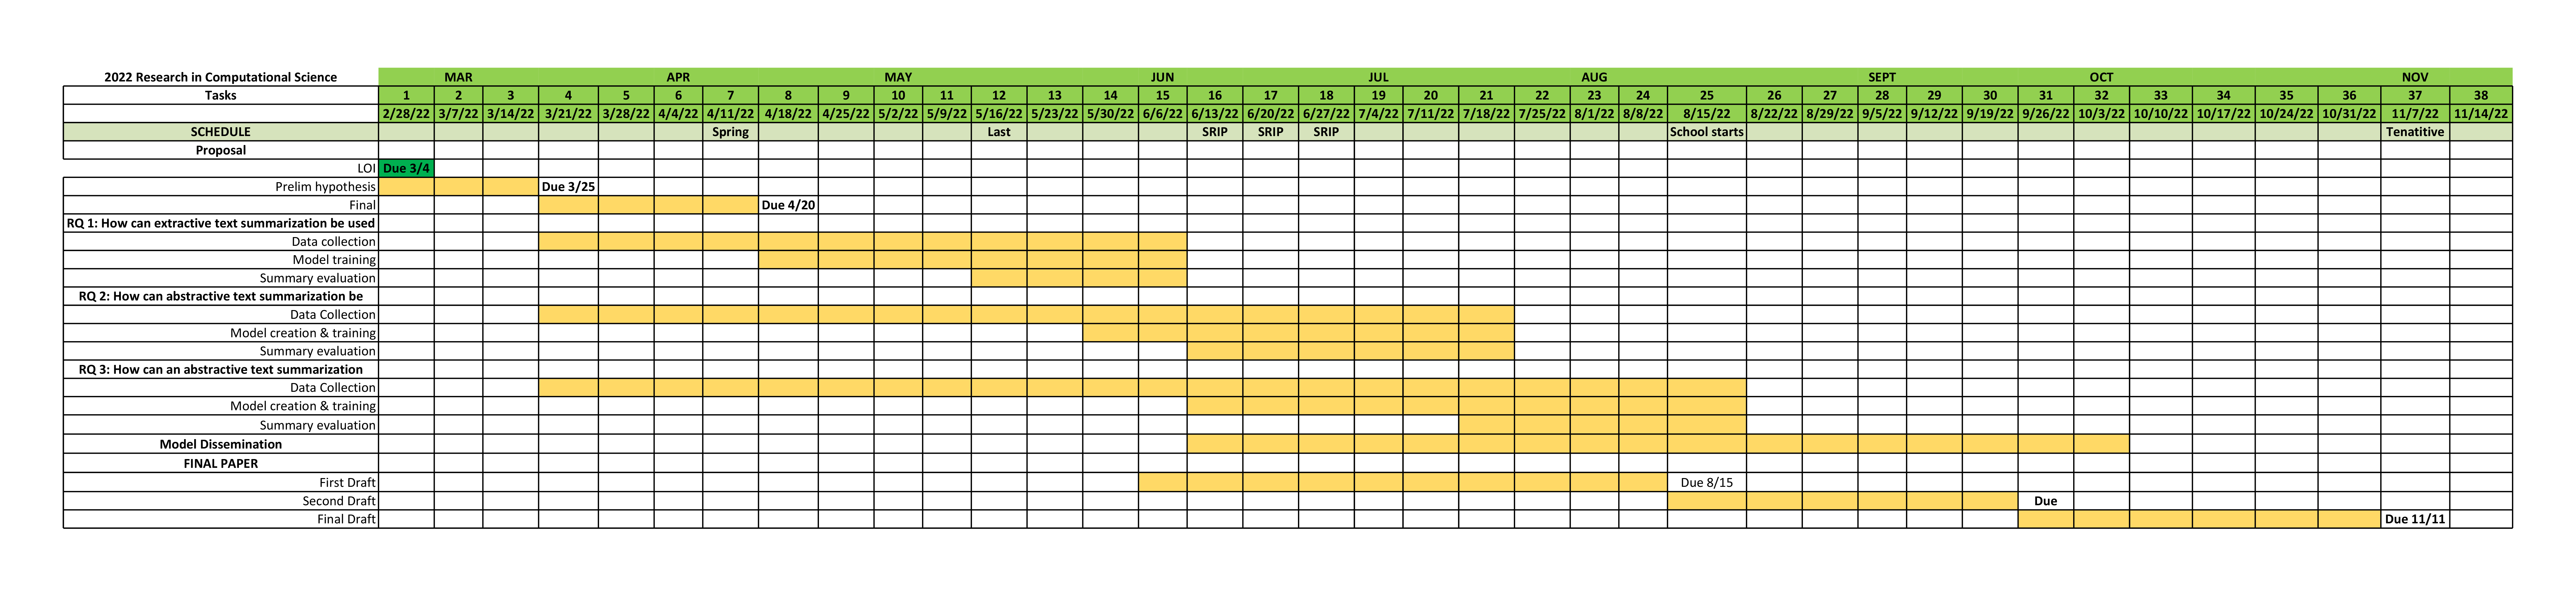
\includegraphics[scale=0.05]{images/RCompSci2022GANTTChart (1).png}
    \caption{First draft of GANTT chart}
    \label{fig:gantt}
\end{figure}

\subsection{Tuesday, March 22, 2022}
Today I wrote the intellectual merits part of my preliminary proposal and also created an outline for the rest of the proposal. I also wrote the overview, dissemination, and finished the project personnel part of my proposal.

\subsection{Wednesday, March 23, 2022}
\begin{itemize}
    \item Came up with the name of my project: Machine Learning for Research Paper Simplification (MAL-
REPS)
    \item Wrote the overview of my project
    \item Exapnded on RQ1, 2, and 3 and added them to the proposal.
    \item Rationale for MALREPS
    \item Theoretical framework (started on it)

\end{itemize}



\subsection{Thursday, March 24, 2022}
I FINISHED WRITING MY PRELIMINARY PROPOSAL TODAY AND I TURNED IT IN!!!

\subsection{Friday, March 25, 2022}
Today I watched the video \href{https://www.youtube.com/watch?v=7kLi8u2dJz0}{"What is BERT? | Deep Learning Tutorial 46 (Tensorflow, Keras & Python)"} which goes over what BERT is and how to use it.

How can similarity be captured between different words? You can look at features between different words.
\begin{enumerate}
    \item Look at various features of the input text
    \item Create vectors of the values of each feature of each input text (called a word embedding)
    \item The model figures out each feature on its own (we don't know how ML works)
    \item BERT can generate contextualized embedding (unlike something such as Word2Vec), which means that the same word used in two different contexts will generate different embedding
\end{enumerate}

\subsection{Saturday, March 25, 2022}
Today I read over the TensorFlow hub documentation for how to preprocess and use the BERT model itself to create text embeddings. There are also many other models that can be used for word embeddings, such as ulmfit, electra, gtr, and more.

I also found a pretty interesting research paper that describes when BERT was created. I will probably read this paper in the upcoming days. The paper is here \href{https://arxiv.org/abs/1810.04805}{BERT: Pre-training of Deep Bidirectional Transformers for Language Understanding
}

The BERT model source code is \href{https://github.com/google-research/bert}{here on GitHub}.

\subsection{Sunday, March 27, 2022}
Today I wrote code that is able to preprocess text and generate word embeddings using BERT from the tensorflow hub website.

\section{Week of March 28, 2022}
\subsection{Monday, March 28, 2022}
Today I watched the video \href{https://www.youtube.com/watch?v=hOCDJyZ6quA}{Text Classification Using BERT & Tensorflow | Deep Learning Tutorial 47 (Tensorflow, Keras & Python)}. Notes from my video are below:

\begin{itemize}
    \item Downsampling, take the smallest number of rows based on each category. Ex: x has 100 samples while y has 300 samples. Take 100 rows of x and 100 rows of y to train the data.
    \item sklearn.model\_selection has a function called train\_test\_split that is able to split pandas data frame into training and test data
    \item The code from this video is on \href{https://github.com/codebasics/deep-learning-keras-tf-tutorial/blob/master/47_BERT_text_classification/BERT_email_classification-handle-imbalance.ipynb}{GitHub}
    \item sklearn.metrics.pairwise has a function called cosine\_similarity that can measure the similarity between two sentences that have been turned into a vector with BERT.
    \item Metrics in ML don't actually have an effect on the model train (that works on the loss function)
    \item you can only rely on accuracy when using a BALANCED dataset
    \item Confusion matrix shows correct and wrong predictions
\end{itemize}

I sent emails to:
\begin{itemize}
    \item Mr. Miller (Leveraging BERT)
    \item Dr. Srivastava (NLP UNC)
\end{itemize}

\subsection{Tuesday, March 29, 2022}
Word2Vec is a method of turning a sentence into a sequence of numbers, because comoputers can only understand numbers. I watched the video: \href{https://www.youtube.com/watch?v=hQwFeIupNP0}{What is Word2Vec? A Simple Explanation | Deep Learning Tutorial 41 (Tensorflow, Keras & Python)}

\begin{itemize}
    \item Embeddings are created via neural networks.
    \item ``Self-supervised", meaning that there isn't necessarily a correct output
    \item Words that have a similar meaning result in similar vectors.
\end{itemize}

The way word embeddings are created:
\begin{enumerate}
    \item Take a fake problem (such as fill in a missing word in sentence--BERT)
    \item Solve it using neural network
    \item Word embedding is created as a SIDE EFFECT 
\end{enumerate}

I also began reading the research paper: \href{https://arxiv.org/pdf/2109.06838.pdf}{Employing Proverbs in Context as a Benchmark for Abstract
Language Understanding}

\begin{itemize}
    \item Email sent to Dr. Bansal (mbansal@cs.unc.edu)
    \item Email sent to Dr. Dhingra (bdhingra@cs.duke.edu)
    \item Email sent to Dr. Barzilay (regina@csail.mit.edu)
\end{itemize}

\subsection{Wednesday, March 30, 2022}
Today I prepared the Python workshop that I will be presenting to the class on Thursday (3/31). The topics that I created code for are:
\begin{itemize}
    \item Basic Python syntax
    \item data science (tables, datasets, plotting, analyzing data)
    \item sentiment analysis
    \item Classifying movie reviews
\end{itemize}

\subsection{Thursday, March 31, 2022}
Today I presented the Python workshop in class. I think that it went really well, except for a few parts where Mr. Gotwals said that R was better than Python O-O

Emails sent today:
\begin{itemize}
    \item Dr. Chaturvedi (snigdha@cs.unc.edu)
    \item Dr. Woodsend (email failure)
\end{itemize}

\subsection{Friday, April 1, 2022}
In class today, we learned about file management, UNIX commands, and how computers really work. I think that taking out ``since you're an expert, I was wondering...." makes my emails sound more professional. I also don't know whether or not keeping the line ``I would like to talk to you about my own research questions and hear your thoughts on them" is a good way to ask when emailing potential mentors.

Emails sent today:
\begin{itemize}
    \item Dr. Wiseman (swiseman@duke.edu)
    \item Dr. Wills (lisa@cs.duke.edu)
\end{itemize}

\subsection{Saturday, April 2, 2022}
Emails sent to today:
\begin{itemize}
    \item Dr. Fahlman (sef@cs.cmu.edu)
    \item Dr. Singh (singh@ncsu)
\end{itemize}

\subsection{Sunday, April 3, 2022}
Emails sent to mentors today:
\begin{itemize}
    \item Dr. Berg (berg.tamara@gmail.com)
    \item Dr. Frederking (ref@cs.cmu.edu)
    \item 
\end{itemize}

\section{Week of April 4}
\subsection{Monday, April 4, 2022}
Today we went over things that we need to change for our preliminary proposals. I think for me, the main things will be the work plan and the background sections. Today I edited the parts that were easier to fix, such as contractions and such.

\subsection{Tuesday, April 5, 2022}
No progress today. I had a datathon, and our team got honorable mention (2nd place)

\subsection{Wednesday, April 6, 2022}
Emails sent: 
\begin{itemize}
    \item Dr. Oliva (joliva@cs.unc.edu)
    \item Ms. Bauer (lbauer6@cs.unc.edu)
\end{itemize}

I also finished all of the ``easy" edits on my NSF proposal today. I added graphics, citations, fixed typos, expanded contractions, etc. I also started giving more background for machine learning.

\subsection{Thursday, April 7, 2022}
Today I drafted more mentor emails and read research papers regarding them. I also responded to mentor emails. Most of the mentors are rejecting me, and I don't know if I will be able to find a mentor for SRIP.

\subsection{Friday (April 8, 2022) - Sunday (April 10, 2022)}
I was at the Technology Student Association (TSA) State conference for this weekend. I didn't get a chance to work on RCompSci materials during this time.

\section{Week of April 11, 2022}
\subsection{Monday, April 11, 2022}
Today I emailed more mentors and set up a meeting with Vaibhav (PhD student) from NCSU. Vaibhav's work doesn't directly deal with NLP, but I wonder if I might be able to look into something with him.

\subsection{Tuesdday, April 12, 2022}
Today I finshed all the changed I need from my preliminary proposal. I will be proofreading and trying to lower my hemingway score in the next few days.

\subsection{Wednesday, April 13, 2022}
Today I put my final proposal through hemingway and grammarly and fixed grammatical errors. I turned in my final proposal today. I also got on a call with Vaibhav from NCSU, and he wants to work with me. However, he is more interested in social media text simplification rather than research paper text simplification.

\subsection{Thursday, April 14, 2022}
Today I set up my GitHub repository where I will be creating an npm package that adds word explanations to sentences.


\subsection{Friday, April 15, 2022}
Today I got the first draft of my word substitutions working. The endpoint is /api/simplify and it adds simplified definitions to the ends of words.

\subsection{Saturday, April 16, 2022}
Today I thought about possible projects that I might want to complete with the 3rd year graduate student at NCSU. My ideas are below:

\begin{itemize}
    \item Doing text simplification on reddit posts to extract the general gist of information, this would allow more information to be spread on reddit, as people don't usually read super long posts.
    \item Doing summary creation on reddit posts to generate a summary of a single post
\end{itemize}

\subsection{Sunday, April 17, 2022}
No progress today, I was enjoying Spring break with my family.

\section{Week of April 18, 2022}
\subsection{Monday, April 18, 2022}
Today I fixed an error on the API endpoint where if you gave it an unkown word that wasn't in the dictionary, it would cause an error. Now, it no longer throws an error. I also created an NPM package for my project.

\subsection{Tuesday, April 19, 2022}
Today I watched the video: \href{https://www.youtube.com/watch?v=TQQlZhbC5ps}{Transformer Neural Networks - EXPLAINED! (Attention is all you need)}, which explained the paper Attention is all you need. This paper introduced the concept of transformers.

\begin{itemize}
    \item Vector sequence models produce a variable length output
    \item Sequence vector models produce a fixed length output
    \item Sequence to sequence models produce variable length output
    \item Normal recurrent neural networks are VERY slow to train. Each word is passed in one after the other (time)
    \item With transformers, the embeddings are created all at once (simultaneously).
    \item Attention vectors are created using transformers, which represents how important a word is
\end{itemize}

\subsection{Wednesday, April 20, 2022}
Today I watched the video \href{https://www.youtube.com/watch?v=XcZGKAF5zxg}{Text Summarization in SpaCy and Python}. They took the entire document and found the most common words that appeared the most number of times throughout, and then chose the sentences with the highest occurrences  of the words with the most occurrences. This method of extractive text summarization may work, but I think it would be worth it to compare this method of text summarization on research papers compared with the k-means clustering method and and seeing which performs better.

\subsection{Thursday, April 21, 2022}
Today I watched the video \href{https://www.youtube.com/watch?v=Yo5Hw8aV3vY}{Automatic Summarization using Deep Learning | Abstractive Summarization with Pegasus}. They used Pegasus to perform extractive text summarization on news articles and wikipedia articles but also SCIENTIFIC RESEARCH. The abstractive model here works really well, and I think that I will be able to use this model in my project as well. It is able to simplify an abstract of a research paper really easily. They also have a model that is specially trained with the PubMed dataset, which may create better abstractive text summarizations.

\subsection{Friday, April 22, 2022}
Today I installed gnuplot on my computer and signed up for a supercomputing account for our labs next week. 

\subsection{Saturday, April 23, 2022}
No progress today, I was at a competition all day.

\subsection{Sunday, April 24, 2022}
Today I prepared for my meeting with Vaibhav, who said that he wants to do research with me related to social media and hot topics (asian hate crimes, LGBTQ+ rights, racism, the Black Lives Matter movement, etc). The topic that I have the most hope for in my work with Vaibhav is doing text simplification on reddit posts about Asian hate crimes.

\section{Week of April 25, 2022}
\subsection{Monday, April 25, 2022}
Today I got with Vaibhav and Mr. Gotwals together on a call. This call went super well, Vaibhav has agreed to formally mentor me over the summer. Additionally, the lab PI, Dr. Singh, is allowing me to go to NC State over the summer each day to work in their lab. I think the most important step for me to now do is finding subreddits that we might be able to do text simplification on and contain relevant stories about asian hate crimes.

\subsection{Tuesday, April 26, 2022}
Today I created a list of subreddits that I thought we might be able to find posts about personal experiences relating to asian racism and hate from. However, many of the Reddit posts that I found that were in these subreddits were either news stories or just contained a link to a different news article. This made it very difficult to actually perfom text simplification, unless we went to the link contained within the post and scraped the information from there. Looking at ICWSM papers though, I think 

\begin{itemize}
    \item It's a Thin Line Between Love and Hate: Using the Echo in Modeling Dynamics of Racist Online Communities (for dataset of racism)
    \item Analysis of Twitter Users' Lifestyle Choices using Joint Embedding Model (for subject extraction)
\end{itemize}

\subsection{Wednesday, April 27, 2022}
Today I read over Gotwals guide for supercomputing. Today we also went over the introductory slides on the Bridges 2 supercomputer.

\subsection{Thursday, April 28, 2021}
Today I was able to debug the code I had with pegasus for abstractive text summarization. I think that we should also be able to use GPTJ for this summarization as well. My next step will be figuring out how to deploy this model onto an endpoint so any API call can make the request.

\subsection{Friday, April 29, 2022}
Today we did gnuplot in class. I also created a ML model using the huggingface API and Allen NLP that is able to take in a long piece of text, a question, and the number of bullet points that the user wants to get back, and we give them a summary. I deployed this on gradio, and comes with an API endpoint.

\subsection{Saturday, April 30, 2022}
Today I created a frontend for the API endpoint that I created yesterday. https://verste-ovz2hei6k-ganning127.vercel.app/simplify

\subsection{Sunday, May 1, 2022}
Today I watched another \href{https://www.youtube.com/watch?v=4Bdc55j80l8}{video} explaining the paper ``Attention is all you need", which was the video that invented transformers, a type of neural network.
\begin{itemize}
    \item encoder - maps input sequence to a continuous representation of the input, which holds all the info from previous inputs
    \item decoder - generates output while keeping in mind all the previous outputs
\end{itemize}

The steps that transformers use:
\begin{enumerate}
    \item Input embedding - create vectors (numerical representations of the sentence). An example is shown in ``embedding.png".
    \item Multi-headed attention: how words are associated with each other (if a single word occurs more often with another word)
\end{enumerate}

Convolutional neural networks are typically used for images, as they scan a window of frames. Before transformers, recurrent neural networks were used (looked at each word at a single time). They process words in order, so start from word 1 and end at final word. This had several issues: by the time you got to the end of the paragraph, the network already forgot what was at the beginning, can't do parallel processing. 

Transformers are much better, they can keep attention, be trained in parallel, are are much faster to train. Transformers look at positional encodings and SELF-attention. Positional embeddings meant that each word had its own vector based on its position in the sentence, so the position meaning was built into the word itself. While attention has been around for a long time, the new item about this paper was SELF attention.

\section{Week of May 2, 2022}
\subsection{Monday, May 2, 2022}
Today we went over fundamentals of machine learning, including supervised and unsupervised learning, cluster analysis, PCA, dimensionality reduction, and more. We also went through three mathemtica notebooks on machine learning. We talked about how various models could be used to classify artwork to an author, show the network of relationships between trump and russia, and show how we can attribute a work of writing to an author.

\subsection{Tuesday, May 3, 2022}
Today I was looking for datasets related to racism. I found a CSV file of 56k tweets from Donald Trump about various topics that he has talked about. Also, I found a paper titled \href{https://ojs.aaai.org/index.php/ICWSM/article/view/18050/17853}{X-Posts Explained: Analyzing and Predicting Controversial Contributions in Thematically Diverse Reddit Forums} that has a good looking reddit dataset, but I cannot access it. I emailed the researcher there, in hopes of getting the dataset. 

\subsection{Wednesday, May 4, 2022}
Today I watched the video: \href{https://www.youtube.com/watch?v=jgKj-7v2UYU}{Easy Custom NLP T5 Model Training Tutorial - Abstractive Summarization Demo with SimpleT5}, which is a open source python package (Simple T5) that can be custom trained for your own dataset. I think for my project, I could use Simple T5 to train my own model for abstractive text summarization using various models from huggingface. 

\subsection{Thursday, May 5, 2022}
I am struggling to find research papers that relate to my topic of subject extraction from racist reddit posts. Thus, I also cannot find many datasets with this purpose either. Some other possible ways to go with this might be fake news detection. 

Today in class we did cluster analysis with machine learning.

\subsection{Friday, May 6, 2022}
Today in class we went over clustering techniques using R. This is how k-means clustering works:
\begin{enumerate}
    \item Plot all data points on an appropriate representation (graph, number line, etc)
    \item Put k number of cluster points directly on the representation just chosen (the best number for k can be chosen through the elbow technique)
    \item Assign each point to the nearest cluster based on euclidean distance. 
    \item Move each cluster to the middle of all of the data points assigned to it
    \item Repeat until the cluster points do not move anymore
\end{enumerate}

I also met with my mentor today. We are probably not going to go with the racism idea because there are not enough data sets out there that I was able to find that related to racism. For the next week, before we meet, we will each be looking over various papers and find a paper where the topic interests us.

\subsection{Saturday, May 7, 2922}
No progress today. I am studying for my AP Calculus BC exam.

\subsection{Sunday, May 8, 2922}
No progress today. I am studying for my AP Calculus BC exam.

\section{Week of May 9, 2022}
\subsection{Monday, May 9, 2022}
Today I began working on the summer report presentation that we will be giving to the rest of the group. I am a little unsure about what I will be doing in the summer still, research wise, because we are still deciding on and finalizing our idea. However, it will likely be something to do with machine learning and text simplification on social media posts. Vaibhav is more into social media posts and I am more into text simplification, so we will meet in the middle.

\subsection{Tuesday, May 10, 2022}
Today I kept working on the summer report presentation that I will be giving to the group. I am still stuck on trying to figure out a topic that we will work on, but I think that I will be reading various research papers from ASONAM, WEbScie, The web conference conferences because they are related to social media. To find accepted papers for each conference, I can search NAME + ``Accepted Papers"

\subsection{Wednesday, May 11, 2022}
Today I added some sections to my summer report (api endoint, and already published website) and finished up and prepared planning for what I am going to say for these Summer Reports.

\subsection{Thursday, May 12, 2922}
Today I read over papers from the ASONAM conference. I can't find many promising papers yet about topics that I'm interested in though. It was also very difficult to find papers from the ASONAM conference.

\subsection{Friday, May 13, 2022}
Today I looked at papers from the WEBSCI conference, which has papers that seem more promising than the one I looked at yesterday. Here are a couple of papers that I might explore further.

\begin{itemize}
    \item \href{https://arxiv.org/abs/2102.03870}{"Short is the Road that Leads from Fear to Hate": Fear Speech in Indian WhatsApp Groups}. Coded in Python, their code is at \href{https://github.com/hate-alert/Fear-speech-analysis}{github.com/hate-alert/Fear-speech-analysis}
    \item \href{https://arxiv.org/abs/2004.04046}{“Go eat a bat, Chang!”: On the Emergence of Sinophobic Behavior on Web Communities in the Face of COVID-19}
     \item \href{https://arxiv.org/pdf/2011.00449.pdf}{Improving Cyberbully Detection with User Interaction}
\end{itemize}

\subsection{Saturday, May 14, 2022}
Today I read the paper, “Short is the Road that Leads from Fear to Hate”: Fear Speech in Indian WhatsApp Groups. In text preprocessing, they only kept tweets that were in English and Hindi, covering over 70\% of the data. To filter out spam messages, a high precision lexicon set was used to remove spam. Then, they removed emojis, stop words, and URLs using regex. The multilingual tokenizer CLTK was used to tokenize sentences. 

The purpose of the paper was to identify fear speech messages against Muslims on whatsapp.

Annotations were made by humans to decide whether or not a post actually depicted hate speech.

Docanno can be used for humans to annotate texts

\textbf{Results}
\begin{itemize}
    \item The lifespan of a fear speech message was longer than that of a non fear speech message.
    \item If we are going to ask people from outside NCSSM/NC State to help us with our research, the response rate will likely be very low.
\end{itemize}

\subsection{Sunday, May 15, 2022}
The paper, “Go eat a bat, Chang!”: On the Emergence of Sinophobic Behavior on
Web Communities in the Face of COVID-19 is about confirming that anti-asian behavior and hate speech actually did increase due to COVID-19.

Datasets were collected from Twitter using the Streaming API and 4chan.

\textbf{Ideas}
I'm thinking that for my RCompSci project, we might be able to do something related to confirimg the prescence of something related to Covid-19? Maybe not directly related to text simplification anymore.

Today I also read the paper "Improving Cyberbullying Detection with User Interaction", which aims to model the behavior of those who cyberbully others through MULTIPLE comments posted, not just one.

We could do asian american racism detection. Comparing the reach of posts and such that are racist towards Asian Americans compared to all other posts on a platform such as Twitter.


\section{Week of May 16, 2022}
\subsection{Monday, May 16, 2022}
Today I met with Vaibhav about our RCompSci project. He was busy last week so this week we will all read papers and talk about them on friday to discuss possbile project ideas that we might want to pursue together.

I also read the paper \href{https://dl.acm.org/doi/pdf/10.1145/3485447.3512128}{Early Identification of Depression Severity Levels on Reddit
Using Ordinal Classification}, which is about classifying depression levels into 4 levels, instead of a binary classification of yes/no.

This was their model architechture:
\begin{figure}
    \centering
    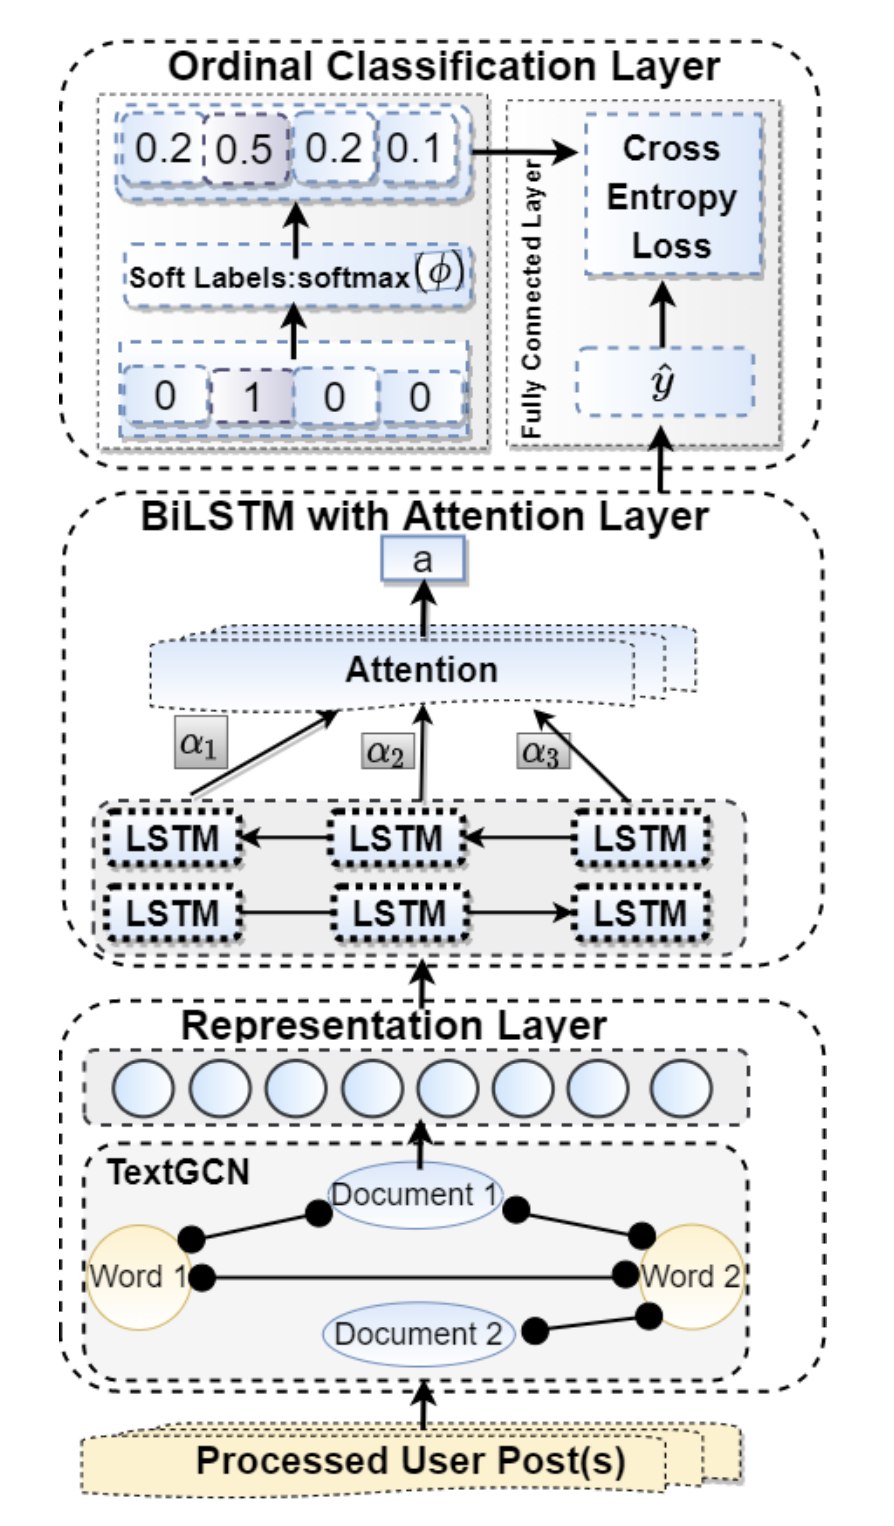
\includegraphics[scale=0.5]{images/id_depress_arch.png}
    \caption{Caption}
    \label{fig:my_label}
\end{figure}

\subsection{Tuesday, May 17, 2022}
Today I read the paper \href{https://arxiv.org/pdf/1703.04009v1.pdf}{Automated Hate Speech Detection and the Problem of Offensive Language∗}, which attempted to classify hate speech from Twitter. Their model accuracy was around 91\%, but when they tested the model on testing data, it only had an accuracy of around 41\%, which may suggest overfitting. A few key takeaways:

\begin{itemize}
    \item Logistic regression was used to do dimensionality reduction on the data
    \item scikit-learn and SVMs were used to classify tweets ad hate speech/not hate speech.
\end{itemize}

Today I also looked at the code from "Deep Learning Models for Multilingual Hate Speech Detection". They have their dataset on \href{https://github.com/hate-alert/DE-LIMIT}{github.com/hate-alert/DE-LIMIT} as well!

\subsection{Wednesday, May 18, 2022}
Today I signed up for a research gate account. In class we went over how to do summer research and I think that one of my weaknesses is definitely needing to speak up more, instead of always being shy.

Reddit posts can be extracted using the \href{https://praw.readthedocs.io/en/stable/}{PRAW API}.

Today I also read the paper ``Identification of Disease or Symptom terms in Reddit to Improve Health Mention Classification", which is about trying to identify posts where users are discussing health conditions rather than using disease and symptom terms for other conditions. This is known as Health mention classification (HMC).

An F-1 score tests a binary model's accuracy on a dataset. The model in this paper only had an F-1 score of 75\%.

\subsection{Thursday, May 19, 2022}
Today I met with Vaibhav again. We both agreed that going for the idea of extracting the specific sentences from fear speech containing messages would be a good idea. 

We need to try and look for patterns in the fear speech messages. For the message mentioned in the paper the order of fear speech is as follows:
\begin{enumerate}
    \item Citing something from history (using numbers or dates)
    \item Spreading fear through any means (misinformation, scaring others, etc). THIS IS THE SENTENCE THAT WE WANT TO EXTRACT.
    \item Asking others to share the message
\end{enumerate}

I have emailed two of the authors of this paper asking for access to their full dataset, as the one currently mentioned in the paper only contains about 8k tweets out of the full 27.

ALSO TODAY WAS THE LAST DAY OF CLASSSESSSS WOOOO!!! 

I think that tomorrow I will be looking at \href{https://raw.githubusercontent.com/hate-alert/Fear-speech-analysis/master/Data/fear_speech_data.json}{more of the fear speech JSON} file and trying to find more datasets.

\subsection{Friday, May 20, 2022}
Today I tried to find more datasets online about fear speech. While I didn't find many datasets that related to fear speech, I did find some that were more targeted towards hate speech, such as the \href{https://huggingface.co/datasets/hate_speech_offensive}{hugging face dataset}.

\subsection{Saturday, May 21, 2022}
When looking at the fear speech dataset that I mentioned on Friday, there doesn't really seem to be a pattern in which the fear speech sentence itself is happening in. However:
\begin{itemize}
    \item Many of the fear speech sentences appear with numbers in them (Example: "Jamaat-e-Islami has more resources than Pakistan, 70+ bank accounts, 350 mosques, 300 madrasas and 4500 crores Islam = terrorism")
    \item Many fear speech sentences also have emojis around the sentence (Example: "[EMOJI]  * * It is a district with a population of about 8 lakhs. Muslims * constitute * 70\% of the population here. This is the same district from where 3 Muslims went to * Syria * to be admitted to * ISIS *."), ("The cure for terrorism is not to kill the terrorist ✊  but to close his factory."),
\end{itemize}

\subsection{Sunday, May 22, 2022}
Toady I wrote a short Python script that turns the JSON file from the github into a more readable CSV file format. Also, there doesn't look to be too much patterns regarding the sentences right before / after the hate speech sentences specifically, but many of them do cite numbers / statistics and use emojis


\subsection{Monday, May 23, 2022}
Today I wrote more of the script and added sections that performed sentiment analysis on the text. Here are my observations:
\begin{itemize}
    \item Fear speech generally has more shares than regular posts
    \item Average length of a fear speech post is longer
    \item Fear speech has a lower average sentiment and is much more radical than normal speech.
\end{itemize}

Patterns in fear speech sentences:
\begin{itemize}
    \item First couple of sentences set the premise for the rest of the information
    \item Next couple sentence is provoking you and trying to get you to hate a certain community. Sentences that provoke directly target another community.
    \item Last the couple of sentences call to action or addressses the reader directly. Conclusion sentences are usually indirect but are implying something.
\end{itemize}

Process to going going about doing this
\begin{enumerate}
    \item manually annotate each sentence to separate the parts of (premise, provoking, call to action)
    \item train the model on input features of this sentence. the target for our model will be our annotation.
    \item Can we build a model that predicts the conclusion based on the provoking sentences?
\end{enumerate}

TODO: Read 10-15 more stories and discuss whether or not the sentence types that we discussed are present.

\subsection{Tuesday, May 24, 2022}
No progress today. I had my calculus final exam today.

\subsection{Wednesday, May 25, 2022}
Today I annotated 4 stories. They were mostly following the structure that we already had, which is really good. However, some of them I don't really understand, as they follow India's politics.

\subsection{Thursday, May 26, 2022}
Today I annotated 4 more stories. Today was also move out day so I didn't get much done.

\subsection{Friday, May 27, 2022}
Today I will be meeting with Vaibhav. Before the meeting, I read over some more posts and stories from the fear speech dataset. I finished all the stories that I was supposed to annotate. Here are some questions I did have, howver:

\begin{enumerate}
    \item Some of the ``sentences" don't end with periods, as the grammar in them is incomplete. How should we deal with this?
    \item What are we going to do about posts that have sentences that don't fall into a specific category of sentences that we have?
    \item How are we going to annotate all of these in such a way that a ML model is able to read through them and train itself?
\end{enumerate}

We need to come up with an actual problem statement that gives the ``motivation" behind why we are doing this research, which would allow us to publish this research. We need to be very clear about what work has previously been done. Then we can find gaps and find a problem statement in which we are able to publish papers.

TODO: Also, read more papers for hate speech.

\subsection{Saturday, May 28, 2022}
No progress today. I had a competition all day and it is summer break.

\subsection{Sunday, May 29, 2022}
Today I found some papers that related to hate speech and fear speech. I think that I will be reading the following papers in the days to come:

\begin{itemize}
    \item \href{https://sci-hub.hkvisa.net/10.1145/3232676}{A Survey on Automatic Detection of Hate Speech in Text}
    \item \href{https://aclanthology.org/W12-2103.pdf}{Detecting Hate Speech on the World Wide Web}
    \item \href{https://arxiv.org/abs/1712.06427}{Detecting Hate Speech in Social Media}
    \item \href{https://sci-hub.hkvisa.net/10.1109/ATSIP.2018.8364512}{On the use of pitch-based features for fear emotion detection from speech}
    \item \href{https://www.isca-speech.org/archive_open/sp2004/sp04_205.pdf}{F0 and pause features analysis for Anger and Fear detection in real-life spoken dialogs}
\end{itemize}

\section{Week of May 30, 2022}
\subsection{Monday, May 30, 2022}
Today I am going to read over the papers that I said I would read over yesterday. The first paper, \textbf{Survey on Automatic Detection of Hate Speech in Text} points out that there is a lack of data about hate speech, automatic techniques for hate speech detection is not available, creates a definition for hate speech:

\begin{itemize}
    \item Hate speech has specific targets (ethnic origin, religion, other)
    \item Hate speech is to incite violence or hate amongst a group
    \item Hate speech is used to attack or diminish another group
\end{itemize}

The most common algorithms used to detect hate speech are SVM, random forests, and decision trees. This paper just provided a background on the work that was previously done.

The paper \textbf{Detecting Hate Speech on the World Wide Web} focuses on creating a method to automatically classify hate speech from regular text with 94\% precision. They noted that:

\begin{itemize}
    \item hate speech uses a small set of high frequency stereotypical words
    \item they used an SVM to classify hate speech from non hate speech.
\end{itemize}

The paper \textbf{On the use of pitch-based features for fear emotion detection from speech} and \textbf{F0 and pause features analysis for Anger and Fear detection in real-life spoken dialogs} focuses on detecting emotion through a person's spoken word, which isn't really about machine learning lol.

\subsection{Tuesday, May 31, 2022}
The paper, \textbf{A Survey on Hate Speech Detection using Natural Language Processing} defines hate speech as something that \emph{ any communication that disparages a person or a group on the basis of some characteristic such as race, color, ethnicity, gender, sexual orientation, nationality, religion, or other characteristic}. Below are some methods usually used in hate speech detection:
\begin{itemize}
    \item Bag of words: Supervised classification technique. Very simple, bu requires that the same predictive words that appear in the training data must appear again in the testing data.
    \item Brown clustering has been used to assign individual words to produce hard clusters. 
    \item Sentiment analysis is sometimes used, as a negative sentiment is said to usually be a hate speech message.
    \item Bayesian Logistic Regression
    \item Hate speech must be read in context, as some sentences by themselves might not be hate speech, but when taking into context the site / environment in which they were posted, they might be hate speech then.
    \item When classifying hate speech from non-hate speech, SVMs are mainly used.
    \item Data for hate speech detection is usually collected from Twitter, Yahoo!, Formspring, Whisper, and Xanga.
\end{itemize}

\subsection{Wednesday, June 1, 2022}
The original paper we read, \textbf{Short is the road that leads from fear to hate: fear speech in indian whatsapp groups} had several results regarding basic analysis between fear speech and regular speech: 
\begin{itemize}
    \item Fear speech typically lasts longer (is continously seen by more people) than regular speech
    \item Fear speech generally has more shares per post than regular texts.
    \item Emojis were more often used in fear speech than regular texts.
    \item They got around an MAX 83\% accuracy. Could we be able to build on this?
\end{itemize}

\textbf{Possible problem statement:} Infering what the people are trying to say from provoking sentences. Vaibhav says that each type of provoking sentences tries of convey a different type of fear.




1. how does this beenefit anyone for publication - benefits people by making things more black and white. also add what type of fear they are inducing. Based on each sentence in a post, we can predict multiple inferences 

for example, if the sentence relates to previous rulers, it might be trying to say that they were atrocious

2. are we generating the conclusion or are we extracting it? 
    a. do drawing conclusions for every single sentences
    b. first do data annotation
    
Processing:
a. phase where me and vaibhav go through and see the red sentences
b. do data annotation and break the dataset into multiple sentences. classify 
c. come up with around 3 category labels for each sentence.

Next Steps:
1. create a new sheet with shuffled rows (do not modify original)
2. do top 20 fear speech and mark sentences with their categories (they need to be red)
3. do around 3 labels
4. do not look at Vaibhav's sheet

\subsection{Thursday, June 2, 2022}
Today I came up with the categories that I will be looking for in the provoking sentences. They are:
\begin{itemize}
    \item Fear about politics (stuff about political leaders, elections)
    \item Fear about religion (items about how a certain religion is bad or that they will do something)
    \item Fear about terrorism or violence  (items about conflicts, deaths)
\end{itemize}

Each provoking sentence may take on multiple labels. 

\subsection{Friday, June 3, 2022}
Today I annotated 3 posts from the fear speech dataset. Most of the posts I've realized that only contains sentences from the same category.

\subsection{Saturday, June 4, 2022}
I just realized that I have been annotating posts from normal speech instead of fear speech. That is quite annoying lol. However, I did notice something.

\begin{itemize}
    \item Normal speech posts usually have one type of provoking sentence, whether that be politics, religion, or terrorism/violence.
    \item Fear speech posts usually have around 1-2, types of provoking sentences
\end{itemize}

\subsection{Sunday, June 5, 2022}
I annotated around 8 more posts today. Tomorrow I will be reading about more papers relating to fear speech and hate speech.

\subsection{Monday, June 6, 20222}
Today I read around 3 more fear speech (long) posts from the dataset that we collected. Most of these posts were very confusing for me to understand, as many had references to Indian figures who I do not know.

\subsection{Tuesday, June  7, 2022}
Today I read over the code of the paper ``HateXplain: A Benchmark Dataset for Explainable Hate Speech Detection", which created a new dataset that created a dataset with:
\begin{itemize}
    \item Label: whether or not the piece of text is hate speech
    \item Targets: the target community of the piece of text (i.e. African Americans)
    \item Text: the piece of text itself. This piece of text also contains an annotated portion that was the que for the annotator to choose hate speech / normal / offensive speech.
\end{itemize}

The dataset they used is \href{https://github.com/hate-alert/HateXplain/blob/master/Data/dataset.json}{on github}.

I also learned that the differenece between hate speech and offensive speech was that hate speech is more threatening and includes a call to violence / action, when offensive speech degrades another group.

\subsection{Wednesday, June 8, 2022}
Today I read over the actual paper ``HateXplain: A Benchmark Dataset for Explainable Hate Speech Detection". The introduction section just details previous work that has been done and how that fails to meet the model the paper created's standards. The introduction also gives a brief overview of their methods and what they did.

To evaluate their code, they used the F-1 score, accuracy, macro F1-score, and AUROC score.

\subsection{Thursday, June 9, 2022}
Today I will meet with Vaibhav to discuss our progress so far.


\begin{itemize}
    \item \textbf{Possible problem statement}: Sentences written about fear speech are indirect, and that's why we need to make a system to identify the real intentions behind writing that sentence.
    \item There already has been a paper that identifies fear speech messages
    \item However, they haven't specified what type of fear (or provoking) is being shown 
    \item What the paper found fearful seems provoking to us, rather than fearful.
    \item Just improving the accuracy might not be enough.
    \item \textbf{Our contributions}: our annotated dataset, model (training and such)
\end{itemize}

In our cause, if we label the sentences for types of provoking, this model can be deployed on an online platform and this allows companies to mark those sentences as the type of provoking.

TODO:
\begin{itemize}
    \item Have a more thought out motivation (who will be helped, why are we doing this)
    \item Split up each post into individual sentences and then we begin annotating (only fear speech) and populate into new google sheet
    \item Find more data on fear speech (maybe scrape some from twitter with keywords such as ``terrorist")
    \item Find conferences that we can submit to in Sep / Oct (\href{https://www.junglelightspeed.com/the-top-10-nlp-conferences/}{here}
\end{itemize}

\subsection{Friday, June 10, 2022}
Today I wrote out the motivation for our research tasks on \href{https://docs.google.com/document/d/17kLWPe7UvaFoTWG4jR4-Zsl5Ngrt6Gf5Pqt5q5fmRsw/edit}{this google doc}.

\subsection{Saturday, June 11, 2022}
Today I wrote a short Python script that will turn the data we originally had for the dataframe into individual sentences.

The Python script is on \href{https://colab.research.google.com/drive/1SiPwRhosjSFBRKsibU_2UrM60fwUtp9I?usp=sharing}{Google Colab}. However, some of the sentences on here are just single letters / numbers. They're not actually a full sentence.

\subsection{Sunday, June 12, 2022}
Today I created a list of conferences that I think we should be able to submit to. The Google sheet is linked \href{https://docs.google.com/spreadsheets/d/1xaAznWx4lQz2tLoyNnGAnjFkoCbv78nOoP6YjoFKf5Y/edit#gid=0}{here}.

\section{Week of June 13, 2022}
\subsection{Monday, June 13, 2022}
Today was the first day of SRIP. We went over mentor expectations and orientation material for this program. I also filled out the planner for tomorrow on what I will be working on in the lab.

\subsection{Tuesday, June 14, 2022}
Today I went in person to NCSU for the first time. I mainly worked in the library building (Hunt library) and I further developed the motivation for our research project. I also revamped the script that we had earlier to use nltk's sentence tokenizer instead of just splitting on periods. I worked on a presentation script today because I will be presenting the status of our research project to the grad student's supervisor tomorrow.

\subsection{Wednesday, June 15, 2022}
Today I went to the NCSU lab again with my mentor. I presented my research to the rest of the research group as a check-in. They suggseted that we look into posts not just from Indian WhatsApp groups, but expand into the US by looking at topics such as gun violence. However, it would be too diffitcult to expand our categories to different topics to include gun violence. Both Vaibhav and I agree on not including this data. Things I've done today:

\begin{itemize}
    \item Random sample of 10k sentences from the dataframe
\end{itemize}

\subsection{Thursday, June 16, 2022}
Today I annotated 200 sentences from the individual sentences dataset. After annotation in the morning, I met with Vaibhav in the afternoon to go over annotation and discussions to go over our disagreements. It took us 1.5 hours to go over just 30 posts, which is an average of around 3 minutes / post.

Additionally, I wrote a short python script for fun that classifies provoking sentences from non-provoking sentences. This model achieved a maximum of 68\% testing accuracy.


I also calculated the cohen-kappa score from our differing annotations and got 0.26. This is really low.

\subsection{Friday, June 17, 2022}
Today I met with Vaibhav in the morning to go over the sentences that we annotated. We came up with the rule that everything that is not ``none" MUST be related to religion somehow, as Vaibhav told me that that is how you get accepted into the most conferences. 

I annotated 200 more sentences today, came up with the annotation guide, and also wrote a script that takes all the raw WhatsApp posts and splits them into individual sentences (ALONG with the sentence directly before and after the target sentence). This allows us to provide context when doing annotations. Vaibhav said that there is a method to feed multiple sentences into a machine learning model at once, which is why we areable to do this.

\subsection{Saturday - Sunday, June 18-29, 2022}
No progress these days because I had a hackathon.

\section{Week of June 20, 2022}
\subsection{Monday, June 20, 2022}
Today I annotated around 50 nmore fear speech posts, as well as read over about multi-label classification. The python package simpletransformers has an example of multi-label clssification that I might be able to use on this dataset. I will create a script that attempts to do this tomorrow. I also went to the mentorship break event today and won a ping pong plushie from the tournament.

\subsection{Tuesday, June 21, 2022}
Today I annotated 100 posts for the individual sentences dataset. I also calculated the cohen kappa score in Python, along with the krippendorf alpha score. I will be calculating our fliess kappa score soon.

Our fleiss kappa score was 0.57, which is already much better than the original dataset's fleiss kappa score of around 0.37.

I also annotated 100 more posts this night.

\subsection{Wednesday, June 22, 2022}
Today I looked into the differences between Cohen Kappa annotation scores and Krippendorf alpha scores. I think that for our purposes, Cohen Kappa scores will be better as we area closer to being satisfcatory for that inter-rater agreement than for the krippendorf alpha one.

Additionally, I wrote two scripts that used an SVM and Naive Bayes algorithm to detect for fear speech and got around 84.3\% accuracy. This is higher than the paper got. Additionally, I wrote a method to test this accuracy with any piece of text the user enters.

I also met with my mentor today and we decided to use Cohen Kappa score for inter-rater reliability. Our Cohen Kappa score for some reason is not increasing from yesterday, as we had exxactly 0.53 for both days. I also revised my 300-400 annotations, read over various disagreements, and will be annotating 100 more posts tonight.

\subsection{Thursday, June 23, 2022}
Our annotations from yesterday saw a Cohen Kappa score of 0.53, which was lower than the previous days' 0.59. I met with Vaibahv today to go over our disagreements on the posts, and below are a few important points from our discussions:
\begin{itemize}
    \item If a post is unclear or doesn't have enough information, mark it as none
    \item If a post is not targeted toward a specific religious group (such as politics or general violence), mark it as none
    \item If the before and current sentences are related, then we are able to say that the provocation in the previous sentence is also in the current sentence, as readers will read previous sentence before current sentence in the real world.
\end{itemize}

Today I will be annotating 100 more posts, revising my reviews from 400-450, and reading over the disagreements of annotations so we are on the same page. I will be reading the labels that Vaibhav's were correct and Vaibhav will be reading the labels that I said were correct.


\subsection{Friday, June 24, 2022}
Today I was playing around with the script that does provocative sentence classification again and got around a 68\% accuracy. The original fear speech detection is 84\% accurate. I wrote the overview of my project today, including the contributions that our project will make, a very drafty abstract and introduction, and a timeline of when each step in our project should be done by.

I will annotate 200 more sentences later today and meet with my mentor. Last night, Vaibhav and I's annotation reached a cohen kappa score of around 0.73, which is really good.


I also figured out a way to translate from English --> ASL Gloss. While the model isn't perfect yet, it achieved a BLEU score on average of about 51, which is interpreted as ``Very high quality, adequate, and fluent translations". I'm thinking about making this my second RCompSci project.

\subsection{Saturday, June 25, 2022}
Today I went through the disagreements that Vaibhav and I had from the disagreements from 400-500. 

\subsection{Sunday, June 26, 2022}
Today I annotated 100 more posts from 500-600.

\section{Week of June 28, 2022}
\subsection{Monday, June 27, 2022}
Today I created an API endpoint in Python and deployed it on Heroku that was able to use SVMs to detect for fear speech.

Additionally, I used BERT and keras layers to create a model to attempt multi-class classification.

I also completed my presentation draft (abstract and presentation) and will be reviewing it before I actually record it.

\subsection{Tuesday, June 28, 2022}
Today I reviewed the sentences where we disagreed on the 100 that we discussed yesterday (500-600). I also read over the pixie paper and the concept of using transformers to adapt them to our methods for our paper.
However, the wifi went out yesterday as well, so I wasn't able to work on annotating sentences.


The cohen kappa score for today's annotations was 0.7, which is really good.

I finished filming my presentation and submitted it to NCSSM's SRIP office today!

\subsection{Wednesday, June 29, 2022}
These are the items I worked on today
\begin{itemize}
    \item I read over our disagreements from annotations 600-700 and added the final labels.
    \item Finished annotations for sentences 700-800
    \item Discussed with mentor our about disagreements and calcuated a cohen kappa score of 0.63
    \item Setup our docanno annotation platform for 6000 posts
    \item Read over methods that were previously used for multi-class text classification in Python.
    \item Annotated 100 posts.
\end{itemize}

\subsection{Thursday, June 30, 2022}
Today I:
\begin{itemize}
    \item Created my final RCompSci presentation for SRIP
    \item Practiced my final SRIP presentation
    \item Met w/mentor and discussed on how to label fear speech when it comes up in our annotations
    \item Split up dataset for annotation of fearful vs. provoking
    \item Set up the mturk account and annotation system (however, it only accepts regular text and not emojis, so I'm not sure on what to do with that.
\end{itemize}

\subsection{Friday, July 1, 2022}
Today was the final day of SRIP. I did my RCompSci presentation today in the lecture hall, along with the rest of the RCompSci folks.

\subsection{Saturday, July 2, 2022}
Today I tried to set up AWS MTurk requester sandbox, but it kept giving me errors:

\begin{enumerate}
    \item Each batch can only be 500 rows
    \item Why did it say that it was going to cost me like \$5?
\end{enumerate}

\subsection{Saturday - Sunday, Jul 2 - 3, 2022}
I was sick these days so I wasn't able to get much done.

\section{Week of July 4, 2022}
\subsection{Monday, July 4, 2022}
Today I annotated sentences to be fearful vs. non-fearful. I only annotated sentences where the final label was "none" or "undecided", as we are only looking for posts where the sentence is only fearful and not provoking. If the label was anything else, then it was provoking.

\subsection{Tuesday, July 5, 2022}
Today I met with Viabhav and we went over next steps that we will need to do for our project. We need to annotate sentences that we have marked as oppressive and determine whether or not they are actually oppressive or just fearful. Our points are below:

\begin{itemize}
    \item Only look at fearful vs. not-fearful at only sentences that were marked as oppression.
    \item Send Vaibhav message when I'm done
    \item Annotate 100 posts
\end{itemize}


\subsection{Wednesday, July 6, 2022}
Today I went through and annotated my share of the posts as fearful vs. non-fearful in all posts with "oppression" or "Undecided" as the final label.

\subsection{Thursday, July 7, 2022}
Today I went through the 10k posts with before and afters and annotated 100 posts. I am finished with phase 1.

\subsection{Friday, July 8, 2022}
No progress today. I am waiting on my mentor to finish his annotations.

\subsection{Saturday, July 9, 2022}t
I was completely sick today, so no progress.

\subsection{Sunday, July 10, 2022}
I am meeting with Vaibhav at 9PM to begin our phase 3 annotations. Here are a couple of tools that I've tried in the past for phase 3:

\begin{itemize}
    \item Docanno: clean and visually pleasing UI. however, i've had all anotations completely been wiped twice already because of the app crashing, resulting in a complete loss of data. I don't think this is the most reliable route to go.
    \item Amazon Requester Sandbox: i think the maximum batch size was only 500 annotations? AWS Says: ``Too many input rows. The maximum number of tasks per batch is 500. For more information, please refer to our FAQ."
\end{itemize}

\section{Week of July 11, 2022}

\subsection{Monday, July 11, 2022}
Today I met with Vaibhav and we discussed how we are going to go about phase 3. However, Amazon MTurk wasn't working on the call, so Vaibhav will talk to a few of the people he knows about it and will get back to me in the next few days on how to make MTurk work. 

\subsection{Tuesday, July 12, 2022}
I tried what Vaibhav said about creating an MTurk worker account. I really don't think it is worth the wait to wait 3 days before we can start our annotations. I think I will be starting m phase 3 tomorrow so we don't fall behind.

\subsection{Wednesday, July 13, 2022}
Today I wrote the script that created files of 200 annotations each for Vaibhav and I. I will begin annotations tomorrow.

\subsection{Thursday, July 14, 2022}
Today I annotated 200 posts.

\subsection{Friday, July 15, 2022}
Today I annotated 200 posts.

\subsection{Saturday, July 16, 2022}
Today I annotated 200 posts.

\subsection{Sunday, July 17, 2022}
Today I annotated 200 posts.

\section{Week of July 18, 2022}
\subsection{Monday, July 18, 2022}
Today I annotated 200 posts.

\subsection{Tuesday, July 19, 2922}
Today I annotated 200 posts.

\subsection{Wednesday, July 20, 2022}
Today I annotated 200 posts.

\subsection{Thursday, July 21, 2022}
Today I annotated 200 posts.

\subsection{Friday, July 22, 2022}
Today I annotated 200 posts.

\subsection{Saturday, July 23, 2022}
No progress today.


\subsection{Sunday, July 24, 2022}
Today I annotated 400 posts.

\section{Week of July 25, 2022}
\subsection{Monday, July 25, 2022}
Today I annotated 200 posts.

\subsection{Tuesday, July 26, 2022}
No progress today.

\subsection{Wednesday, July 27, 2022}
Today I annotated 200 posts.

\subsection{Thursday, July 28, 2022}
No progress today.

\subsection{Friday, July 29, 2022}
No progress today.

\subsection{Saturday, July 30, 2022}
Today I annotated 200 posts.

\subsection{Sunday, July 31, 2022}
No progress today.

\subsection{Monday, August 1, 2022}
Today I have finished annotating a fill in posts. Also, I wrote a script that combines all the annotated datasets together.

\subsection{Tuesday, August 2, 2022}
Today I have wrote a script to determine the length / sentiment of sentences in each category. The oppression category seems to have the most negative sentences, and the none category seems to be the most neutral. Posts with none are also the shortest. \ref{fig:ganning_dist} is the distribution of my annotations.

\subsection{Wednesday, August 3, 2022}
No progress today, I went to the beach.

\subsection{Thursday, August 4, 2022}
No progress today, I went to get my drivers license in the morning and I have a flight to SF in the afternoon.

\begin{figure}
    \centering
    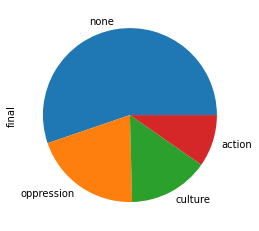
\includegraphics[scale=1]{images/ganning_dist.png}
    \caption{Caption}
    \label{fig:ganning_dist}
\end{figure}

\subsection{Friday, August 5 - Sunday August 7}
No progress. I was in San Francisco.









\newpage
Note: all of my sources are in Mendeley, so I don't have a bibliography here.

\end{document}

\begin{comment}
%Sample LaTeX Code
    % \bibitem{giusti}
    % Giusti, Santochi, \emph{Tecnologia Meccanica e Studi di Fabbricazione}. Casa Editrice Ambrosiana, Seconda Edizione
    % \begin{figure}[H]\centering
    % \includegraphics[scale=0.5]{weintrop.jpg}
    % \caption{Weintrop's Taxonomy}
    % \label{fig:weintrop}
    % \end{figure}

\end{comment}
